\documentclass[11pt,a4paper]{article}
\usepackage[margin=24mm]{geometry}
\usepackage{fontspec}
\setmainfont{Noto Serif CJK SC}[ItalicFont={Noto Serif CJK SC},ItalicFeatures={FakeSlant=0.12}]
\setsansfont{Noto Sans CJK SC}
\setmonofont{DejaVu Sans Mono}[Scale=0.85]
\XeTeXlinebreaklocale "zh"
\XeTeXlinebreakskip=0pt plus 1pt
\usepackage{amsmath,amssymb,amsthm,bm}
\usepackage{graphicx,booktabs,float}
\usepackage[unicode,colorlinks=true,linkcolor=blue!50!black,urlcolor=blue!60!black,citecolor=blue!50!black]{hyperref}
\usepackage{xcolor}
\usepackage{enumitem}
\setlist{nosep,leftmargin=2em}
\setlength{\parindent}{2em}
\setlength{\parskip}{3pt}
\setlength{\emergencystretch}{2em}
\linespread{1.18}
\renewcommand{\figurename}{图}
\renewcommand{\tablename}{表}
\renewcommand{\refname}{参考文献}
\renewcommand{\abstractname}{摘要}
\renewcommand{\proofname}{证明}
\theoremstyle{definition}
\newtheorem{theorem}{命题}
\newtheorem{lemma}{引理}
\newcommand{\F}{\mathrm{F}}
\newcommand{\op}{\mathrm{op}}
\newcommand{\Pol}{\mathcal{P}}
\newcommand{\NumSeeds}{5}
\newcommand{\NumRuns}{140}
\newcommand{\MaxRatio}{0.7400}
\newcommand{\NumViolations}{0}
\newcommand{\SlopeQuadratic}{-0.498}
\newcommand{\SlopeNonconvex}{-0.496}
\newcommand{\SlopeQuadraticMomentum}{-0.481}
\newcommand{\SlopeNonconvexMomentum}{-0.478}
\newcommand{\NeuralMuonTest}{0.002168}
\newcommand{\NeuralAdamTest}{0.008652}
\newcommand{\NSFiveError}{0.512}

\title{Muon 优化器的实现与收敛性验证\\[5pt]\large 从矩阵更新到小型神经网络}
\author{算法与数值实验报告}
\date{}

\begin{document}
\maketitle
\begin{abstract}
Muon 将梯度动量的奇异值重新调整后用于更新矩阵参数。本文实现精确极分解和五阶 Newton--Schulz 两条计算路径，并研究它们能够支持哪些收敛结论。对有下界的光滑目标，在全梯度、无权重衰减、无形状缩放的设定下，证明精确版本的平均梯度核范数具有 $O(T^{-1/2})$ 上界；随后给出包含动量及近似误差的界。数值实验使用两个可解析目标和一个小型神经网络。\NumRuns{} 组独立运行均未违反理论上界，无动量版本的拟合斜率接近 $-1/2$。实验同时展示固定步长振荡和五步近似的残余误差。本文验证的是简化设定下的数学结论及实现行为，不把这些结果扩展为大模型随机训练的收敛保证。
\end{abstract}

\section{引言}
神经网络中的线性层通常以矩阵形式存储参数。若只逐元素调整梯度，更新过程并不直接区分矩阵的主奇异方向与较弱方向。Muon 的做法是先积累动量，再改变更新矩阵的奇异值分布。理想情况下，非零奇异值被替换为 1，保留左右奇异向量。这一操作提供了一个研究矩阵结构与优化行为之间关系的具体入口。

Jordan 等人的公开实现\cite{jordan}采用少量五阶 Newton--Schulz 迭代，并建议主要用于隐藏层矩阵；嵌入、输出层及偏置等参数交给 AdamW。Liu 等人\cite{liu}进一步研究了权重衰减和更新尺度，并将 Muon 用于 Moonlight 模型训练。这些大规模实验说明该方法有应用价值，但训练损失下降与一般性的收敛定理是不同层次的结论。

本文围绕三个问题展开：精确的矩阵更新为什么是下降方向；动量及有限步近似给证明增加了什么条件；实际曲线是否与这些条件一致。以下命题是针对本文设定的自包含推导，不是将文献中的模型训练结果改写成定理。

\section{算法描述}
\subsection{矩阵极分解与更新方向}
设参数 $W\in\mathbb R^{m\times n}$，$r=\min(m,n)$。矩阵内积为
$\langle A,B\rangle=\mathrm{tr}(A^\top B)$。记 $\|\cdot\|_\F$ 为 Frobenius 范数，$\|\cdot\|_*$ 为核范数（奇异值之和），$\|\cdot\|_\op$ 为谱范数（最大奇异值）。

若 $G=U_k\Sigma_kV_k^\top$ 是仅含正奇异值的紧致 SVD，定义
\begin{equation}
  \Pol(G)=U_kV_k^\top,\qquad \Pol(0)=0.
\end{equation}
于是 $\langle G,\Pol(G)\rangle=\|G\|_*$，且
$\|\Pol(G)\|_\F^2=k\le r$。为与紧致极分解的定义一致，代码按数值秩阈值去除零奇异值方向，不向这些方向补上单位更新。

这一方向也解出谱范数约束下的最速下降子问题：
\[
\max_{\|D\|_\op\le1}\langle G,D\rangle=\|G\|_*.
\]
因为 $\langle G,D\rangle=\sum_i\sigma_i u_i^\top Dv_i\le\sum_i\sigma_i$，且取 $D=\Pol(G)$ 时达到等号。这解释了为什么核范数会出现在后面的收敛界中。

Muon 的教学实现如下。令 $G_t=\nabla f(W_t)$，$M_{-1}=0$：
\begin{align}
 M_t&=\beta M_{t-1}+(1-\beta)G_t,\\
 H_t&=G_t+q(M_t-G_t),\quad
 q=\begin{cases}1,&\text{普通动量},\\\beta,&\text{Nesterov 风格混合},\end{cases}\\
 D_t&=\Pol(H_t)\quad\text{或}\quad\operatorname{NS}_K(H_t),\\
 W_{t+1}&=(1-\eta_t\lambda)W_t-\eta_t sD_t.
\end{align}
这里的 Nesterov 风格指作者代码中的混合公式，不额外宣称凸优化中经典 Nesterov 加速法的速率。$s$ 为可选尺度，$\lambda$ 为解耦权重衰减。理论实验使用 $s=1,\lambda=0$。

\subsection{五阶 Newton--Schulz 实现}
先取 $X_0=H/(\|H\|_\F+10^{-7})$。若行数大于列数，先转置以减小 Gram 矩阵的维度。每次计算
\begin{equation}
 A_k=X_kX_k^\top,\qquad
 X_{k+1}=aX_k+(bA_k+cA_k^2)X_k,
 \quad(a,b,c)=(3.4445,-4.7750,2.0315).
\end{equation}
默认 $K=5$。上述系数与固定版本的作者实现一致\cite{code}，本项目用 float64 计算，便于核查误差；不模拟 bfloat16 的数值或 GPU 性能。

需要特别区分“处理奇异值”与“精确正交化”。对应的标量多项式
$p(x)=ax+bx^3+cx^5$ 满足 $p(1)=0.701\ne1$。因此，不能将这组迭代系数当作任意精度极分解求解器，也不能声称增加迭代次数一定降低误差。

\begin{table}[H]
\centering\small
\begin{tabular}{lll}
\toprule
设置 & 更新尺度 $s$ & 本文用途\\\midrule
不缩放 & $1$ & 理论界与矩阵实验\\
Jordan 实现 & $\sqrt{\max(1,m/n)}$ & 小型网络隐藏层\\
Moonlight 约定 & $0.2\sqrt{\max(m,n)}$ & 提供接口，不用于本次曲线\\
\bottomrule
\end{tabular}
\caption{尺度约定并不唯一。更换尺度等价于改变有效步长，不能直接沿用原来的常数。}
\end{table}

\section{收敛性结果与证明}
\subsection{假设及基础不等式}
本节仅研究确定性的全梯度更新。假设 $f$ 可微且有下界 $f_{\mathrm{low}}$，并满足
\begin{equation}
\|\nabla f(X)-\nabla f(Y)\|_\F\le L\|X-Y\|_\F.
\label{eq:smooth}
\end{equation}
记 $\Delta=f(W_0)-f_{\mathrm{low}}$。由线段积分可得下降引理
\begin{equation}
 f(W-\eta D)\le f(W)-\eta\langle\nabla f(W),D\rangle
                  +\frac{L\eta^2}{2}\|D\|_\F^2.
\label{eq:descent}
\end{equation}
具体而言，沿 $W-u\eta D$ 积分梯度差，再用式\eqref{eq:smooth}界定被积项，积分 $\int_0^1u\,du=1/2$ 即得。

\begin{lemma}
任意 $G,H\in\mathbb R^{m\times n}$ 满足
\begin{equation}
 \langle G,\Pol(H)\rangle
 \ge \|G\|_*-2\sqrt r\|H-G\|_\F.
 \label{eq:polar-error}
\end{equation}
\end{lemma}
\begin{proof}
令 $E=H-G$。由 SVD 的定义及 Cauchy--Schwarz 不等式，
\begin{align*}
\langle G,\Pol(H)\rangle
 &=\|H\|_*-\langle E,\Pol(H)\rangle\\
 &\ge\|G\|_*-\|E\|_*-\sqrt r\|E\|_\F\\
 &\ge\|G\|_*-2\sqrt r\|E\|_\F.
\end{align*}
最后一步使用 $\|E\|_*\le\sqrt r\|E\|_\F$。证明同时覆盖零矩阵和秩亏矩阵。
\end{proof}

\subsection{无动量精确版本}
\begin{theorem}
设 $D_t=\Pol(G_t)$，$W_{t+1}=W_t-\eta D_t$，其中 $\eta>0$ 为常数。则
\begin{equation}
 \frac1T\sum_{t=0}^{T-1}\|G_t\|_*
 \le\frac{\Delta}{\eta T}+\frac{Lr\eta}{2}.
 \label{eq:basic}
\end{equation}
若 $\Delta>0$ 并取 $\eta=\sqrt{2\Delta/(LrT)}$，则
\begin{equation}
 \min_{0\le t<T}\|G_t\|_\F
 \le\frac1T\sum_{t=0}^{T-1}\|G_t\|_*
 \le\sqrt{\frac{2Lr\Delta}{T}}.
 \label{eq:rate}
\end{equation}
\end{theorem}
\begin{proof}
将 $\langle G_t,D_t\rangle=\|G_t\|_*$ 和 $\|D_t\|_\F^2\le r$ 代入下降引理，得
\[
 \eta\|G_t\|_*\le f(W_t)-f(W_{t+1})+Lr\eta^2/2.
\]
对 $t=0,\ldots,T-1$ 求和，函数值项望远镜消去，再利用 $f(W_T)\ge f_{\mathrm{low}}$，即得式\eqref{eq:basic}。代入给定步长并使用 $\|G\|_\F\le\|G\|_*$ 即得式\eqref{eq:rate}。
\end{proof}

这是对平均梯度核范数的界，不是对函数值差 $f(W_T)-f_*$ 的界，也没有证明整个参数序列趋于某个点。对固定 $\eta$，式\eqref{eq:basic}留下 $Lr\eta/2$，不能据此宣称梯度最终为零。若 $\Delta=0$，初值已达到下界，可直接停止。

\subsection{带动量的精确版本}
\begin{theorem}
设 $0\le\beta<1$ 固定，$q\in\{1,\beta\}$，并采用前述动量和精确极分解，$s=1,\lambda=0$。令
\[
 C_\beta=\frac12+\frac{2q\beta}{1-\beta}.
\]
则常步长运行 $T$ 步满足
\begin{equation}
 \frac1T\sum_{t=0}^{T-1}\|G_t\|_*
 \le \frac{\Delta}{\eta T}+Lr C_\beta\eta
 +\frac{2\sqrt r\,q\beta\|G_0\|_\F}{T(1-\beta)}.
 \label{eq:momentum}
\end{equation}
取 $\eta=\sqrt{\Delta/(LrC_\beta T)}$ 后，右端为
$2\sqrt{\Delta LrC_\beta/T}+O(T^{-1})$。
\end{theorem}
\begin{proof}
令 $E_t=M_t-G_t$。初始误差为 $E_0=-\beta G_0$。对 $t\ge1$，
\[
E_t=\beta E_{t-1}+\beta(G_{t-1}-G_t).
\]
精确更新的长度不超过 $\eta\sqrt r$，故梯度差范数不超过 $L\eta\sqrt r$。递推展开得
\[
 \|E_t\|_\F\le\beta^{t+1}\|G_0\|_\F
 +\frac{\beta L\eta\sqrt r(1-\beta^t)}{1-\beta}.
\]
求平均并用几何级数求和，得到
\begin{equation}
 \frac1T\sum_t\|E_t\|_\F
 \le\frac{\beta\|G_0\|_\F}{T(1-\beta)}
 +\frac{\beta L\eta\sqrt r}{1-\beta}.
\end{equation}
因为 $H_t-G_t=qE_t$，引理给出
$\langle G_t,D_t\rangle\ge\|G_t\|_*-2q\sqrt r\|E_t\|_\F$。
将其代入下降引理，求和后使用上述平均误差界，整理即得式\eqref{eq:momentum}。
\end{proof}
当 $\beta$ 接近 1 时，该界的常数会增大。因此，本命题说明固定动量参数下的速率阶，不说明动量一定比无动量更快。实验对两种动量设置分别使用其定理给出的步长，图中曲线高低不能用于判断调参后的最优性能。

\subsection{有限步近似能验证什么}
令实际方向为 $D_t$，近似误差为
$\delta_t=\|D_t-\Pol(H_t)\|_\F$。由引理和内积不等式，
\begin{equation}
\langle G_t,D_t\rangle\ge\|G_t\|_*
-2\sqrt r\|H_t-G_t\|_\F-\|G_t\|_\F\delta_t.
\end{equation}
因此，对任意正步长序列，在无衰减、无额外缩放的更新下，
\begin{align}
\frac{\sum_t\eta_t\|G_t\|_*}{\sum_t\eta_t}
\le \frac{\Delta+\sum_t\eta_t B_t}{\sum_t\eta_t},\qquad
B_t={}&2\sqrt r\|H_t-G_t\|_\F+\|G_t\|_\F\delta_t\notag\\
&+\frac{L\eta_t}{2}\|D_t\|_\F^2.
\label{eq:inexact}
\end{align}
证明只需将前一个不等式代入下降引理并求和。代码逐步记录右端各项并核查式\eqref{eq:inexact}。这是包含实测误差的事后界；若不能进一步控制误差项，就不能把它写成五步 Muon 的无条件 $O(T^{-1/2})$ 定理。

\section{仿真设计}
所有矩阵实验使用 $12\times8$ 参数、float64 和种子 $0,\ldots,4$。每条曲线画种子均值，阴影为最小值到最大值的范围，不是置信区间。数据由程序生成，无外部数据下载。

\subsection{可解析目标}
二次问题为
\[
 f(W)=\tfrac12\|\operatorname{diag}(\sqrt h)Q(W-W_\star)\|_\F^2,
\]
其中 $Q$ 为正交矩阵，$h$ 按几何序列分布于 $[1,30]$。故 $L=30$，且 $f_*=0$ 在 $W_\star$ 处达到。初值元素独立服从标准正态分布，目标元素除以 $\sqrt{12}$。

非凸问题为
\[
 f(W)=\tfrac12\sum_{ij}h_i(W_{ij}-W_{\star,ij})^2
       +0.2\sum_{ij}(1-\cos W_{ij}),
\]
其中 $h_i\in[0.02,1]$ 按几何序列取值。可取 $L=1.2$ 和 $f_{\mathrm{low}}=0$。当最小曲率方向的元素为 $\pi$ 时，二阶导数为 $0.02-0.2<0$，因此目标确为非凸。这里的零仅是下界，不声称为最优值。

\subsection{步数、步长与核查指标}
收敛速率实验取 $T\in\{64,128,256,512,1024,2048,4096\}$，比较 $\beta=0$ 与带 Nesterov 混合的 $\beta=0.9$。每个 $T$ 都重新初始化，并按对应命题选择步长。这样避免将一条固定步长轨迹的多个前缀误当成定理中的不同预算实验。指标为
$T^{-1}\sum_{t=0}^{T-1}\|G_t\|_*$，记录更新前的梯度。

另用 2048 步比较固定步长与衰减步长。所有变体共享
$\eta_0=\sqrt{2\Delta/(Lr\cdot2048)}$；衰减设置为
$\eta_t=\eta_0/(1+t/64)^{0.6}$。该实验观察轨迹及式\eqref{eq:inexact}，不用于代替常步长的速率实验。

\subsection{小型神经网络}
网络为 $10\to24\to3$ 的两层 tanh 回归模型，共 339 个参数。固定教师网络生成 512 个训练样本及 256 个独立测试样本，输出噪声标准差为 0.03。损失为均方误差的一半，mini-batch 大小为 64，更新 800 步。

Muon 只更新隐藏层矩阵，设置 $\beta=0.95,K=5$，启用 Jordan 形状缩放、学习率 0.02；偏置和输出层使用学习率 0.003 的辅助 AdamW。对照使用全参数 AdamW，学习率 0.003，两个方法的权重衰减均为 0.01。辅助及对照 AdamW 的参数为 $(\beta_1,\beta_2,\epsilon)=(0.9,0.999,10^{-8})$。两组使用相同初值、样本和每步 batch；学习率预先固定，未根据测试集选择。

这个网络用于检查完整训练流程，不满足前面实验的全部设定，也不是 Transformer 或大语言模型。它不能验证语言建模质量、分布式扩展性或 GPU 加速比。

\section{数值结果与解释}
\subsection{上界及速率}
\begin{figure}[H]
\centering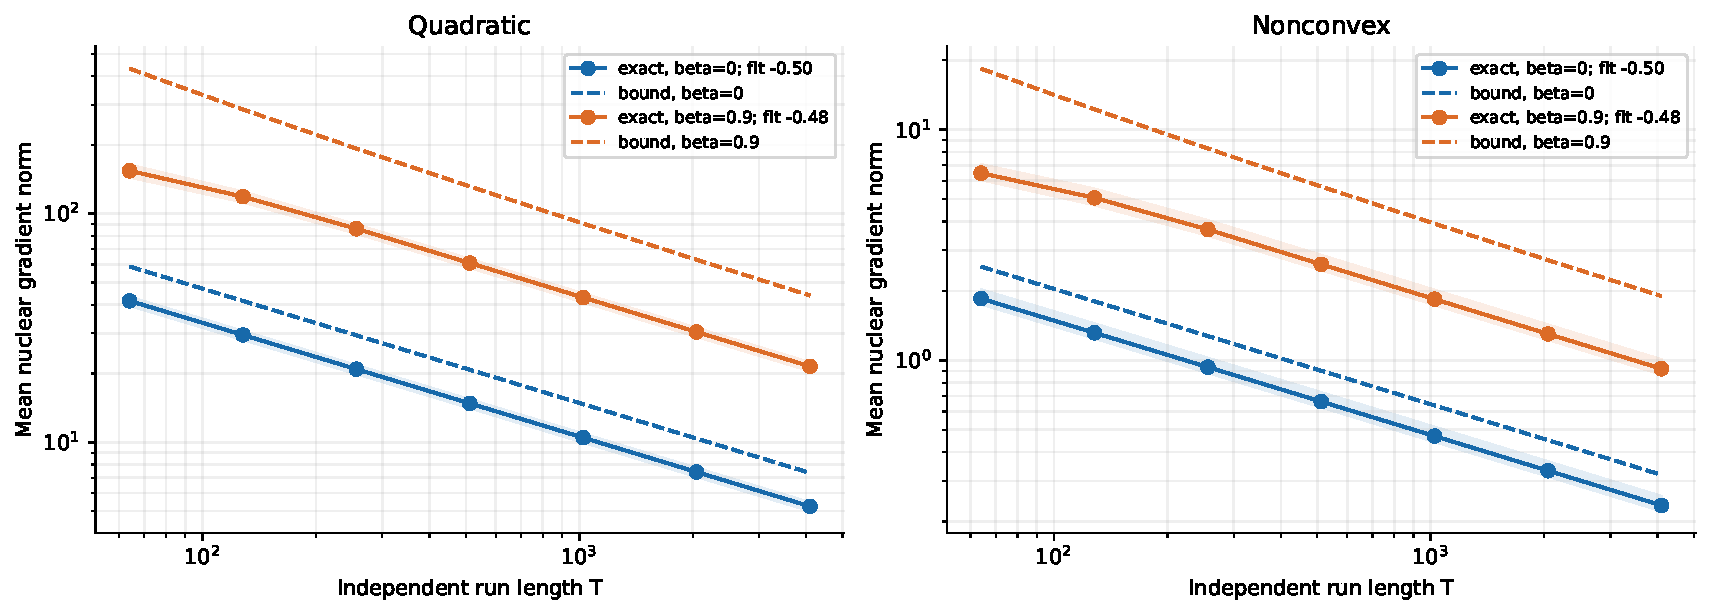
\includegraphics[width=\linewidth]{../results/01_convergence_rate.pdf}
\caption{精确极分解版本的平均梯度核范数与理论上界。实线为实测均值，虚线为对应理论界的种子均值；所有单独运行也逐一检查。}
\end{figure}
共完成 $2\times2\times\NumSeeds\times7=\NumRuns$ 组运行，超过理论上界的次数为 \NumViolations，最大“实测值/上界”为 \MaxRatio。程序还逐步核查下降不等式，允许的误差容限为 $10^{-9}\max(1,f(W_0),\text{bound})$。

对种子均值作 $\log$--$\log$ 最小二乘拟合，无动量版本在二次与非凸问题上的斜率分别为 \SlopeQuadratic、\SlopeNonconvex；带动量版本分别为 \SlopeQuadraticMomentum、\SlopeNonconvexMomentum。结果与有限预算下的 $T^{-1/2}$ 行为一致。有限个点的拟合不能代替证明，也不证明该上界在所有问题上都是紧的。

\subsection{固定步长和近似误差}
\begin{figure}[H]
\centering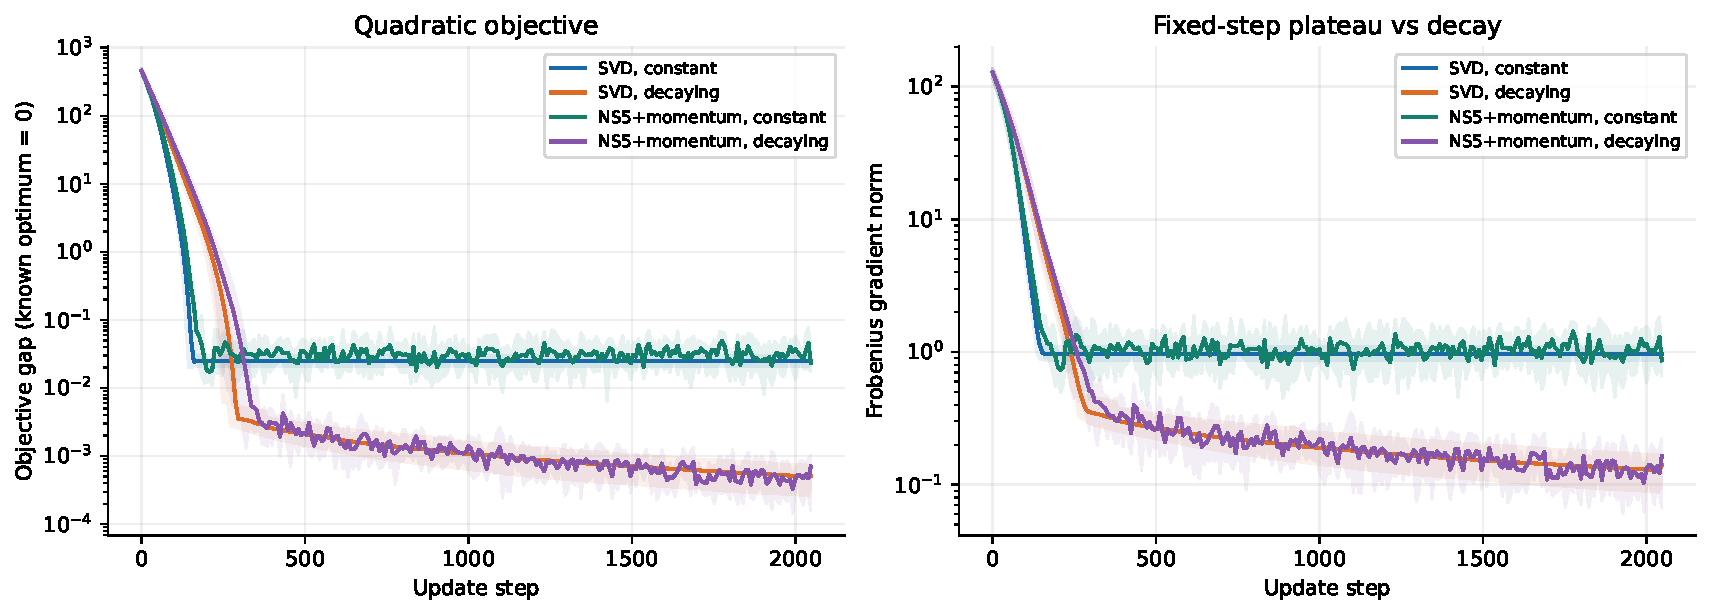
\includegraphics[width=\linewidth]{../results/02_optimization_trajectories.pdf}
\caption{二次问题上的目标值差及梯度范数。衰减步长减小了末期平台。各变体使用相同初始步长，但没有分别做超参数搜索。}
\end{figure}
固定步长精确版本的最终目标值差均值约为 $2.47\times10^{-2}$，衰减后约为 $5.00\times10^{-4}$；五步近似加动量对应约为 $3.75\times10^{-2}$ 与 $3.45\times10^{-4}$。这说明减小步长能在本例中降低末期误差，不等于证明所有非凸问题的参数序列收敛。

\begin{figure}[H]
\centering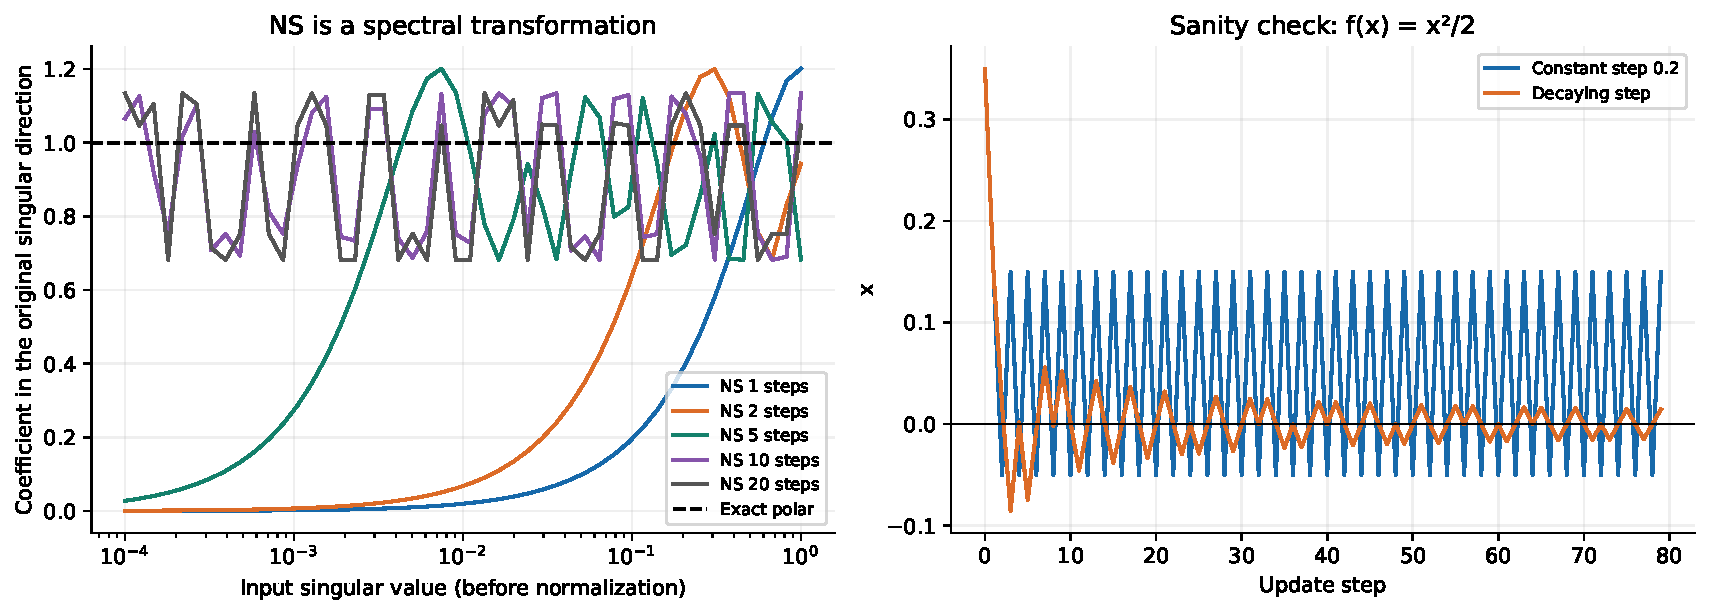
\includegraphics[width=\linewidth]{../results/03_ns_and_step_size.pdf}
\caption{左：对奇异值跨度为 $10^4$ 的对角矩阵进行多项式变换。右：一维强凸二次函数上的符号更新说明固定步长仍可振荡。}
\end{figure}
谱实验中，五步近似相对极分解的 Frobenius 误差为 \NSFiveError；10 步约为 0.202，20 步约为 0.215。更多迭代没有带来单调改善，与 $p(1)\ne1$ 的观察一致。右图取 $x_0=0.35,\eta=0.2$；更新 $x_{t+1}=x_t-\eta\operatorname{sign}(x_t)$ 在经过 0.15 后，于 $-0.05$ 和 0.15 之间来回变化。

\subsection{神经网络训练}
\begin{figure}[H]
\centering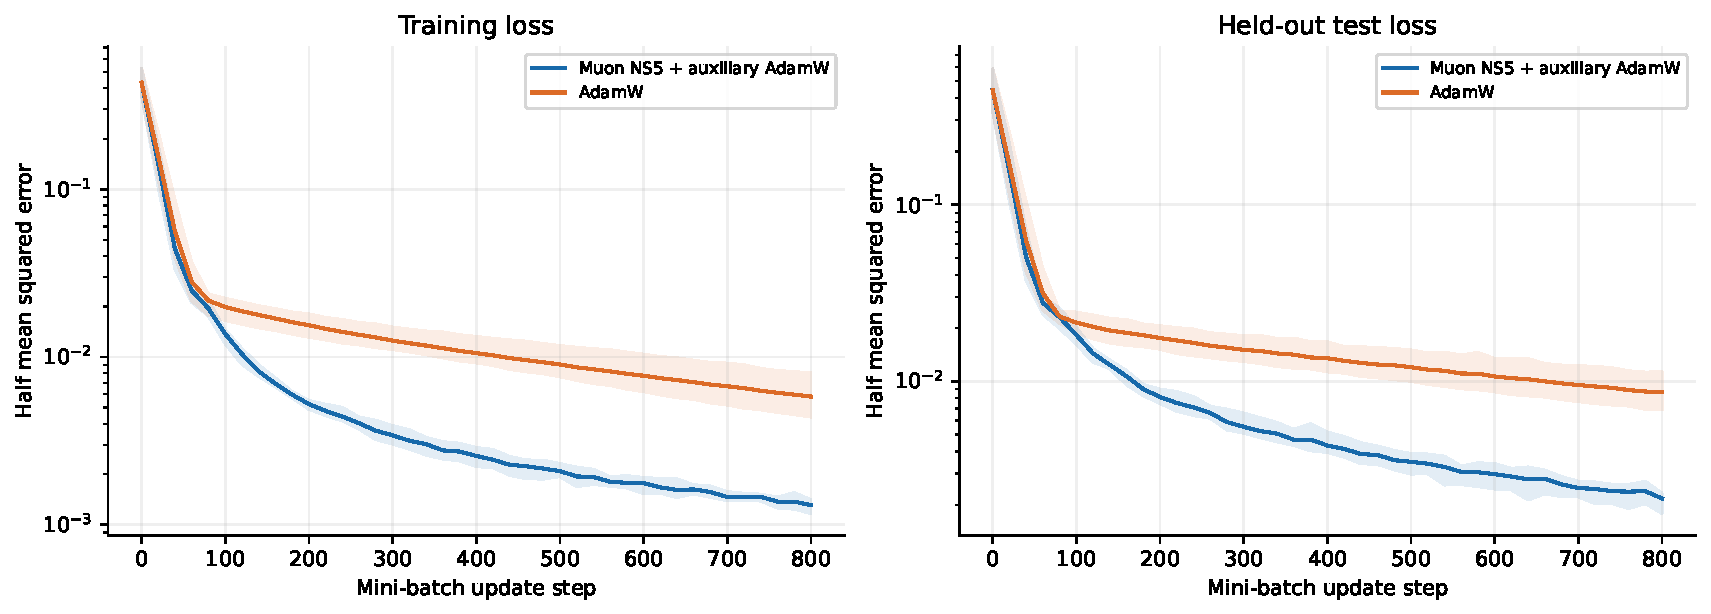
\includegraphics[width=\linewidth]{../results/04_neural_network.pdf}
\caption{合成回归任务上的训练损失与独立测试损失。阴影是五个种子的范围。}
\end{figure}
第 800 步时，Muon 加辅助 AdamW 的测试损失均值为 $\NeuralMuonTest$，全参数 AdamW 为 $\NeuralAdamTest$。前者在这组预设学习率和数据上取得较低误差。由于没有完整的学习率搜索、真实语言任务和计算预算比较，这个结果不支持“Muon 普遍优于 AdamW”的结论。

\section{复现、代码及检查}
项目依赖 Python 3.12、NumPy 2.3.5 与 Matplotlib 3.10.8，不需要 GPU 或 PyTorch。运行以下命令即可重新生成数据和图：
\begin{verbatim}
python -m pip install -r requirements.txt
python -m unittest discover -s tests -v
OPENBLAS_NUM_THREADS=1 OMP_NUM_THREADS=1 \
  python -m muon_study.experiments --output results --seeds 5
cd report
xelatex -interaction=nonstopmode -halt-on-error muon_report.tex
xelatex -interaction=nonstopmode -halt-on-error muon_report.tex
\end{verbatim}
PDF 使用 XeLaTeX、Noto CJK 字体，不依赖外部图片下载。\texttt{results/metrics.tex} 由实验脚本生成，报告的主要汇总指标直接读取该文件。

11 项检查全部通过，覆盖：秩亏矩阵的极分解与核范数恒等式、零梯度、Newton--Schulz 标量多项式、转置路径、动量公式、缩放与衰减、两类目标的有限差分梯度、理论界、所有网络参数组的反向传播、AdamW 首步及非法输入。

\begin{table}[H]
\centering\small
\begin{tabular}{ll}
\toprule
文件 & 内容\\\midrule
\texttt{muon\_study/optimizers.py} & Muon、精确极分解、五阶 NS、辅助 AdamW\\
\texttt{muon\_study/problems.py} & 目标函数、合成数据、手写反向传播\\
\texttt{muon\_study/experiments.py} & 实验、理论界核查、CSV 与图表导出\\
\texttt{tests/test\_core.py} & 11 项数值与功能检查\\
\texttt{results/summary.json} & 实际运行版本、汇总数值、运行时间\\
\texttt{results/*.csv} & 每个种子与每组设置的原始数据\\
\bottomrule
\end{tabular}
\caption{代码与结果文件的对应关系。}
\end{table}

\noindent\textbf{仿真代码入口：}
\href{https://github.com/rou521/optimize-and-game/blob/main/muon_study/optimizers.py}{算法源码（GitHub）}，
\href{https://github.com/rou521/optimize-and-game/blob/main/muon_study/experiments.py}{实验源码（GitHub）}。
完整项目、原始数据、图表和本报告归档于：
\begin{center}\url{https://github.com/rou521/optimize-and-game}\end{center}
在仓库页面选择 \texttt{Code} $\to$ \texttt{Download ZIP} 即可下载全部文件，或使用
\href{https://github.com/rou521/optimize-and-game/archive/refs/heads/main.zip}{完整工程 ZIP 下载链接}。
\texttt{SHA256SUMS.json} 提供项目文件校验值；需要固定版本时，可在 GitHub 文件页面按 \texttt{y} 获取带提交 SHA 的永久链接。

\section{结论}
精确 Muon 的下降性质来自两个矩阵恒等式：梯度与更新方向的内积等于梯度核范数，更新的 Frobenius 范数平方不超过矩阵最小维度。它们给出了简洁的有限步上界。固定动量引入梯度跟踪误差，但在全梯度、光滑目标及适当步长下仍可保留 $T^{-1/2}$ 的速率阶。

实际的五步更新保留了额外近似误差，不能省略这一项后直接套用精确版本的结论。数值实验同时观察到上界成立、固定步长平台和有限步近似误差；这些现象共同说明了理论的适用范围。进一步研究大模型训练时，需要补充随机梯度假设、参数分组、权重衰减和尺度控制，并在语言建模任务上单独验证。

\begin{thebibliography}{9}
\bibitem{jordan} Keller Jordan, Yuchen Jin, Vlado Boza, You Jiacheng, Franz Cesista, Laker Newhouse, Jeremy Bernstein.
\emph{Muon: An optimizer for hidden layers in neural networks}. 2024.
\url{https://github.com/KellerJordan/Muon}.
算法简介与引用信息依据作者仓库 README。
\bibitem{liu} Jingyuan Liu, Jianlin Su, Xingcheng Yao, et al.
\emph{Muon is Scalable for LLM Training}. 2025. arXiv:2502.16982.
\url{https://arxiv.org/abs/2502.16982}.
本文阅读的原文来自
\href{https://github.com/MoonshotAI/Moonlight/blob/c2ad5b20c605086526a179d36901bfc41b52b44b/Moonlight.pdf}{MoonshotAI/Moonlight 作者仓库的论文 PDF（固定版本）}。
\bibitem{code} Keller Jordan et al. \emph{Muon reference implementation: muon.py}.
固定提交：\texttt{f98f1cacc0263b04290753e32be8d498c1efc806}.
\href{https://github.com/KellerJordan/Muon/blob/f98f1cacc0263b04290753e32be8d498c1efc806/muon.py}{GitHub：Muon 固定版本源码}。
\end{thebibliography}
\end{document}
